%% LyX 2.1.4 created this file.  For more info, see http://www.lyx.org/.
%% Do not edit unless you really know what you are doing.
\documentclass[11pt]{article}
\usepackage[latin9]{inputenc}
\usepackage{geometry}
\geometry{verbose}
\usepackage{fancyhdr}
\pagestyle{fancy}
\usepackage{amsmath}
\usepackage{amssymb}
\usepackage{graphicx}
\usepackage{esint}

\makeatletter
%%%%%%%%%%%%%%%%%%%%%%%%%%%%%% User specified LaTeX commands.
\usepackage[margin=0.75in]{geometry} % see geometry.pdf on how to lay out the page. There's lots.
\usepackage{graphicx}
\usepackage{cleveref}
\usepackage{amsmath}
\usepackage{multirow}
\usepackage{listings}
\usepackage{color}
\usepackage{CJK}
\definecolor{mygreen}{RGB}{28,172,0}
\definecolor{mylilas}{RGB}{170,55,241}

\usepackage[latin9]{inputenc}
\usepackage{geometry}
\geometry{verbose}


\makeatletter
\@ifundefined{date}{}{\date{}}
\makeatother

%Fancy-header package to modify header/page numbering 
\usepackage{fancyhdr}
\pagestyle{fancy}
\lhead{\textbf{Ge/ESE 118}} %name of the course
\chead{\textbf{}} %topic of the homework set
\rhead{\textbf{Solution 4}} %number of the homework set
\lfoot{}
\cfoot{}
\rfoot{\thepage}


% Matlab script
\lstset{language=Matlab,%
      %basicstyle=\color{red},
  breaklines=true,%
  morekeywords={matlab2tikz},
  keywordstyle=\color{blue},%
  morekeywords=[2]{1}, keywordstyle=[2]{\color{black}},
  identifierstyle=\color{black},%}
  stringstyle=\color{mylilas},
  commentstyle=\color{mygreen},%
  showstringspaces=false,%without this there will be a symbol in the places where there is a space
  numbers=left,%
  numberstyle={\tiny \color{black}},% size of the numbers
  numbersep=9pt, % this defines how far the numbers are from the text
  emph=[1]{for,end,break},emphstyle=[1]\color{red}, %some words to emphasise
                                                      %emph=[2]{word1,word2}, emphstyle=[2]{style},    
}

\makeatother

\begin{document}

\subsection*{Problem 1 (graded by Yiran) 30 points}


\subsubsection*{(a) - 5 points}

The misfit function 
\begin{eqnarray*}
F(\boldsymbol{m})=\sum_{i}\frac{(d_{i}-g_{i}(\boldsymbol{m}))^{2}}{2\sigma_{d}^{2}}
\end{eqnarray*}


Then, the posterior PDF

\begin{eqnarray*}
P(\boldsymbol{m}|\boldsymbol{d})\propto P(\boldsymbol{d}|\boldsymbol{m})\propto\exp\left(-F(\boldsymbol{m})\right)\approx\exp\left(-F(\boldsymbol{m}_{0})-\frac{\partial F}{\partial\boldsymbol{m}}^{T}(\boldsymbol{m}-\boldsymbol{m}_{0})-\frac{1}{2}(\boldsymbol{m}-\boldsymbol{m}_{0})^{T}\frac{\partial^{2}F}{\partial\boldsymbol{m}\partial\boldsymbol{m}}(\boldsymbol{m}-\boldsymbol{m}_{0})\right)
\end{eqnarray*}
 has the form of a multivariate Gaussian distribution, So the covariance
matrix will be 
\begin{eqnarray*}
cov(\boldsymbol{m})=\left(\frac{\partial^{2}F}{\partial\boldsymbol{m}\partial\boldsymbol{m}}|_{\boldsymbol{m}=\boldsymbol{m}_{0}}\right)^{-1}=\boldsymbol{H}^{-1}
\end{eqnarray*}
Note we want to know covariance matrix when $m_{0}$ is the least
squares solution. 

Using HW2's convention, define 
\begin{eqnarray*}
\hat{G}_{i,k}=\frac{\partial g_{i}}{\partial m_{k}}
\end{eqnarray*}


Then

\begin{eqnarray*}
H\approx\frac{\hat{G}^{T}\hat{G}}{\sigma_{d}^{2}}
\end{eqnarray*}


In HW2, we didn't include the data error in the hessian. So we need
to modify it by dividing $\sigma_{d}^{2}$ when calculate the model
covariance matrix. 

(See MATLAB code) The output model covariance matrix is:
\begin{verbatim}
    0.0101   -0.0123    0.0095    0.0548    
   -0.0123    0.0198   -0.0156   -0.0853     
    0.0095   -0.0156    0.0237    0.1034     
    0.0548   -0.0853    0.1034    0.4985
\end{verbatim}
\selectlanguage{english}%

\subsubsection*{(b)- 5 points}

The covariance matrix calculated here will be similar to the Monte
Carlo simulation in HW2. They should be more and more similar when
$\sigma_{d}\rightarrow0$.

Diagonal element shows the variance of each parameter. The square
root of the diagonal elements gives the standard deviations: $\sigma_{x_{s}}=0.1006$,
$\sigma_{y_{s}}=0.1405$, $\sigma_{z_{s}}=0.1538$, $\sigma_{P}=0.7060$.
The number is very close to that estimated before: $\sigma_{x_{s}}=0.099670,\sigma_{y_{s}}=0.137469,\sigma_{z_{s}}=0.149719,\sigma_{P}=0.691071$.

The off diagonal shows the covariance between parameters. Note also
it's common to change the covariance matrix to correlation matrix
($\rho_{xy}=\frac{\sigma_{xy}}{\sigma_{x}\sigma_{y}}$). The correlation
matrix is:
\begin{verbatim}
    1.0000   -0.8685    0.6127    0.7721    
   -0.8685    1.0000   -0.7200   -0.8598     
    0.6127   -0.7200    1.0000    0.9520     
    0.7721   -0.8598    0.9520    1.0000
\end{verbatim}
\selectlanguage{english}%
we see that there are strong trade-offs between mode parameters. The
strong negative correlation between $x_{s}$ and $y_{s}$, for example,
is also shown in the plot in HW2.


\subsubsection*{(c)- 5 points}

Now 
\begin{eqnarray*}
F(\boldsymbol{m}) & = & \frac{1}{2\sigma^{2}}(\boldsymbol{d}-\boldsymbol{Gm})^{T}(\boldsymbol{d}-\boldsymbol{Gm})
\end{eqnarray*}
where $\sigma=0.1$, and 
\begin{eqnarray*}
\boldsymbol{G} & = & \left[\begin{array}{cc}
\boldsymbol{1} & \boldsymbol{x}\end{array}\right]\\
\boldsymbol{m} & = & [m1,m2]^{T}
\end{eqnarray*}
The Hessian is 
\begin{eqnarray*}
\boldsymbol{H} & = & \frac{1}{\sigma^{2}}\boldsymbol{G}^{T}\boldsymbol{G}
\end{eqnarray*}
and 
\begin{eqnarray*}
cov(\boldsymbol{m}) & = & \boldsymbol{H}^{-1}
\end{eqnarray*}


(see MATLAB code) The output covariance matrix is:
\begin{verbatim}
   1.0e-03 *
    0.3429   -0.0019    
   -0.0019    0.0004
\end{verbatim}
\selectlanguage{english}%

\subsubsection*{(d)- 5 points}

Since in this case, we assume uniform prior, then $P(m|d)\propto P(d|m)$.
The full parameter space calculate the likelihood $P(d|m)$, while
the covariance is calculated from distribution $P(m|d)$. So the error
map in full-parameter-space in HW2, forms an ellipsoid, whose axis
length and rotation angle is all determined by this covariance matrix.
For example, the box containing the error ellipsoid has height/width
ratio about $(500-100)/(2-(-8))\approx4/1$, which is similar to $\sqrt{164.83/0.11213}$.
The off diagnoal is negative, explains the negative slope in HW2.


\subsubsection*{(e)- 5 points}

First calculate the misfit$F(\boldsymbol{m})$ for the full parameter
space.

From Bayesian law and uniform prior,

\begin{eqnarray*}
P(\boldsymbol{m}|\boldsymbol{d}) & \propto & P(\boldsymbol{d}|\boldsymbol{m})\\
 & \propto & \exp(-F(\boldsymbol{m}))\\
\end{eqnarray*}


Normalize the pdf so its integral over the model space equals 1.

\begin{eqnarray*}
P(\boldsymbol{m}|\boldsymbol{d}) & = & \frac{\exp(-F(\boldsymbol{m}))}{\int\exp(F(\boldsymbol{m})d\boldsymbol{m})}
\end{eqnarray*}


\begin{eqnarray*}
P(m_{1},m_{2}|\boldsymbol{d}) & = & \frac{\exp(-F(m_{1},m_{2}))}{\int\int P(m_{1},m_{2}|d)dm_{1}dm_{2}}
\end{eqnarray*}


The marginals are: 
\begin{eqnarray*}
P(m_{1}|d) & = & \int P(m_{1},m_{2}|d)dm_{2}\\
P(m_{2}|d) & = & \int P(m_{1},m_{2}|d)dm_{1}\\
\end{eqnarray*}


We can approximate the integral with rectangle method ($\int f(x)dx=\sum_{i}f(x_{i})\triangle x$).


\subsubsection*{(f)- 5 points}

By definition

\begin{eqnarray*}
\sigma_{m_{i}}^{2}=E[m_{i}^{2}]-(E[m_{i}])^{2} & = & \int p(m_{i}|d)m_{i}^{2}dm_{i}-\left(\int p(m_{i}|d)m_{i}dm_{i}\right)
\end{eqnarray*}


(see MATLAB code)$\sigma_{m1}=0.0185$, $\sigma_{m2}=0.0006$, which
are equal to square root of the diagnoal elements of the covirance
matrix calculated in (c).

\clearpage{}


\subsection*{Problem 2 (graded by Toby) - 15 points}


\subsubsection*{(a)}

The posterior probability is given by 
\begin{equation}
p(\mu|\v{x})\propto\left(\sum_{k=1}^{N}(x_{k}-\mu)^{2}\right)^{-\frac{N-1}{2}}=\exp\left(-\frac{N-1}{2}\ln\left[\sum_{k=1}^{N}(x_{k}-\mu)^{2}\right]\right).
\end{equation}
Minima of $F$ maximize the probability density function. We have
that \begin{subequations} 
\begin{align}
F(\mu) & =\frac{N-1}{2}\ln\left(\sum_{k=1}^{N}(x_{k}-\mu)^{2}\right),\\
\frac{\partial F}{\partial\mu} & =-(N-1)\frac{\sum_{k=1}^{N}(x_{k}-\mu)}{\sum_{k=1}^{N}(x_{k}-\mu)^{2}}\\
\frac{\partial^{2}F}{\partial\mu^{2}} & =(N-1)\frac{N\sum_{k=1}^{N}(x_{k}-\mu)^{2}+2\sum_{k=1}^{N}(x_{k}-\mu)}{\left(\sum_{k=1}^{N}(x_{k}-\mu)^{2}\right)^{2}}.
\end{align}
\end{subequations} Because $\exp$ and $\ln$ are monotonic functions,
we therefore need to find the minimum of the sum of the equared error
(least-squares) 
\begin{equation}
\sum_{k=1}^{N}(x_{k}-\mu)^{2}=0.
\end{equation}
Taking the derivative with respct to $\mu$ and setting it to zero
yields the minimum $\mu_{0}$ 
\begin{equation}
\mu_{0}=\frac{1}{N}\sum_{k=1}^{N}x_{k},
\end{equation}
which is the sample mean of the data. For the standard deviation $\sigma_{\mu}$
we expand $F$ to second order and insert $\mu_{0}$, i.e., 
\begin{equation}
p(\mu|\v{x})\propto e^{-F(\mu)}\approx e^{-F(\mu_{0})-\frac{1}{2}F''(\mu_{0})(\mu-\mu_{0})^{2}},
\end{equation}
For the second derivate at the best fit solution we have 
\begin{equation}
\frac{\partial^{2}F}{\partial\mu^{2}}=\frac{N(N-1)}{\sum_{k=1}^{N}(x_{k}-\mu)^{2}}.
\end{equation}
The standard deviation $\sigma_{\mu}$ then amounts to 
\begin{equation}
\sigma_{\mu}=\frac{1}{F''(\mu_{0})^{1/2}}=\frac{S}{\sqrt{N}},
\end{equation}
where 
\begin{equation}
S=\sqrt{\frac{1}{N-1}\sum_{k=1}^{N}(x_{k}-\mu_{0})^{2}}
\end{equation}
is the sample variance of the data.


\subsection*{(b)}


\subsubsection*{Formal general proof}

We prove that an orthogonal matrix $\mathbf{Q}$ does not impact the
norm of a vector $\v{x}$. Then $\mathbf{Q}$ is called an isometry.
If the length of an arbitrary vector is preserved, $\mathbf{Q}$ must
be a rotation matrix, because only rotations leave the length of vector
unchanges. To prove this, we use the $\mathcal{L}_{2}$-norm of an
arbitrary vector $x$ and the fact that for orthogonal matrices, we
have $\v{Q}^{-1}=\v{Q}^{T}$. We can then write 
\begin{equation}
\ltwo{\v{x}}=\v{x}^{T}\v{x}=\v{x}^{T}\mathbf{1}\v{x}=\v{x}^{T}\v{Q}^{-1}\v{Q}\v{x}=\v{x}^{T}\v{Q}^{T}\v{Q}\v{x}=(\v{Q}\v{x})^{T}(\v{Q}\v{x})=\ltwo{\v{Q}\v{x}}.
\end{equation}
Since the left hand side and the right hand side are equal, we have
shown that the lengths are equal and unchanged under orthogonal transformations.


\subsubsection*{Simple proof in 2D}

In two dimensions, we have that $\v{Q}=(\v{e}_{1}\,\,\v{e}_{2})$,
where $\v{e}_{i}$ are the column vectors of $\v{Q}$. They are orthonormal.
Now, operating $\v{Q}$ on the column vector $\v{x}=(x_{1},\,x_{2})^{T}$
gives 
\begin{equation}
\v{x}'=\v{Q}\v{x}=x_{1}\v{e}_{1}+x_{2}\v{e}_{2},
\end{equation}
which is the representation of the vector $\v{x}'$ in the eigenbasis
of $\v{H}$. Because the $\v{e}_{i}$ have length 1, the vector $\v{x}'$
has length $\sqrt{x_{1}^{2}+x_{2}^{2}}$. But this is the length of
$\v{x}$ as well. So $\v{x}$ and $\v{x}'$ are of the same magnitude.
Formally, we have 
\begin{equation}
\ltwo{\v{x}'}=\v{x}'^{T}\v{x}'=x_{1}^{2}\v{e}_{1}^{T}\v{e}_{1}+x_{2}^{2}\v{e}_{2}^{T}\v{e}_{2}+2x_{1}x_{2}\v{e}_{1}^{T}\v{e}_{2}=x_{1}^{2}+x_{2}^{2}=\v{x}^{T}\v{x}=\ltwo{\v{x}}.
\end{equation}
This is exactly (!) the same logic as in the general proof but applied
explicitly for the two-dimensional problem.


\subsubsection*{Simple explanation}

Because $\v{x}^{T}\v{H}\v{x}=\text{const}.$ defines an ellipse when
$\v{H}$ is symmetric, where the eigenvectors of $\v{H}$ define the
principle axes of the ellipse, we can think of $\v{Q}\v{x}$ as a
rotation into a coordinate system aligned with these principle axes.
This can be seen from $\v{x}'^{T}\v{\Lambda}\v{x}'=\text{const}$,
which also defines an ellipse, but with the principle axes aligned
with the coordinate axes (since $\v{\Lambda}$ is diagonal).


\subsubsection*{(c)}

We need to show that $\sigma_{x}^{2}=\frac{B}{AB-C^{2}}$. We are
deadling with an integral of the form \begin{subequations} 
\begin{align}
\sigma_{x}^{2} & =\frac{\int dxdy\,x^{2}\exp\left(-\frac{1}{2}\v{x}^{T}\v{A}\v{x}\right)}{\int dxdy\,\exp\left(-\frac{1}{2}\v{x}^{T}\v{A}\v{x}\right)}\\
 & =\frac{\int\d{x}\d{y}\,x^{2}\exp\left(-\frac{1}{2}(Ax^{2}+2Cxy+By^{2})\right)}{\int\d{x}\d{y}\,\exp\left(-\frac{1}{2}(Ax^{2}+2Cxy+By^{2})\right)}\\
 & =\frac{\int\d{x}\d{y}\,x^{2}\exp\left(-\frac{1}{2}(A-C^{2}/B)x^{2}-\frac{1}{2}B(y+Cx/B)^{2}\right)}{\int\d{x}\d{y}\,\exp\left(-\frac{1}{2}(A-C^{2}/B)x^{2}-\frac{1}{2}B(y+Cx/B)^{2}\right)}\\
 & =\frac{\int\d{x}\,x^{2}\exp\left(-\frac{1}{2}(A-C^{2}/B)x^{2}\right)}{\int\d{x}\,\exp\left(-\frac{1}{2}(A-C^{2}/B)x^{2}\right)}
\end{align}
\end{subequations} If we set $\sigma^{2}=1/(A-C^{2}/B)$, we arrive
at 
\begin{equation}
\sigma_{x}^{2}=\frac{\int\d{x}\,x^{2}\exp\left(-\frac{1}{2}x^{2}/\sigma^{2}\right)}{\int\d{x}\,\exp\left(-\frac{1}{2}x^{2}/\sigma^{2}\right)}
\end{equation}
, which as we have seen in previous homework sets and solutions implies
\begin{equation}
\sigma_{x}^{2}=\langle x^{2}\rangle=\sigma^{2}=\frac{1}{A-\frac{C^{2}}{B}}=\frac{B}{AB-C^{2}}.
\end{equation}
The hint was used in step 3. In step 4 we integrated out the $y$-dependence
because the integration boundaries of $\pm\infty$.


\subsection*{Problem 3 (graded by Kangchen) - 35 points}


\subsubsection*{(a) - 5 points}

It is not reasonable to assume that all model parameters have constant
priors (-$\infty$ to $\infty$). For $x_{s}$and $y_{s}$, we should
know that it cannot be too far from where the volcano is. For $z_{s}$
which we defined as depth, it must be positive. For P which is related
to pressure, we know that it must be positive too.


\subsubsection*{(b) - 5 points}

We can incorporate this information as a prior by multiplying our
likelihood $P(\{d_{k}\}|m)$ by a prior for model $P\{m\}$. In this
case we will use a gaussian distribution for model parameter $p$
with $\mu=35$ and $\sigma=6$.

\begin{eqnarray*}
P(\boldsymbol{m})=e^{-\frac{1}{2}(\frac{p-\mu}{\sigma})^{2}}\\
P(\boldsymbol{m}|\{d_{k}\})=P(\{d_{k}\}|\boldsymbol{m})P(\boldsymbol{m})\\
P(\boldsymbol{m}|\{d_{k}\})=e^{-F(\boldsymbol{m})}e^{-\frac{1}{2}(\frac{p-\mu}{\sigma})^{2}}\\
P(\boldsymbol{m}|\{d_{k}\})=e^{-F(\boldsymbol{m})-\frac{1}{2}(\frac{p-\mu}{\sigma})^{2}}
\end{eqnarray*}



\subsubsection*{(c.i) - 5 points}

\begin{eqnarray*}
\int_{v_{1}}^{v_{2}}{P(\phi)d\phi}=\int_{v_{1}}^{v_{2}}{\frac{1}{\phi}dv}=\ln(\phi_{2})-\ln(\phi_{1})\\
\int_{kv_{1}}^{kv_{2}}{P(\phi)dv}=\int_{kv_{1}}^{kv_{2}}{\frac{1}{\phi}dv}=\ln(k\phi_{2})-\ln(k\phi_{1})\\
=\ln(k)+\ln(\phi_{2})-\ln(k)-\ln(\phi_{1})\\
=\ln(\phi_{2})-\ln(\phi_{1})
\end{eqnarray*}


So $P(\phi)=\frac{1}{\phi}$ satisfies scale independent criterion.


\subsubsection*{(c.ii) - 5 points}

We can again incorporate this information as a prior in our expression
for $P(\boldsymbol{m}|\{d_{k}\})$ by multiplying it times our likelihood
(just like in part b). Our expresssion becomes:

\begin{eqnarray*}
P(\boldsymbol{m}|\{d_{k}\})=e^{-F(m)}\frac{1}{p}
\end{eqnarray*}



\subsubsection*{(d) - 5 points}

We want to incorporate both independent pieces of information into
our prior. In this case we can multiply the two priors together. Our
new expression becomes:

\begin{eqnarray*}
P(\boldsymbol{m}|\{d_{k}\})=\frac{1}{p}e^{-F(\boldsymbol{m})}e^{-\frac{1}{2}(\frac{p-\mu}{\sigma})^{2}}
\end{eqnarray*}


Let's plot the two priors separately and then together to see which
information dominates the result. Figure 2 is the Gaussian prior.
Figure 3 is the scale independent prior. Figure 4 is their combination.
We can see that the Gaussian prior is scaled by the scale invariant
prior, but still mainly retains it's shape and thus dominates the
result.

\begin{figure}
\centering{}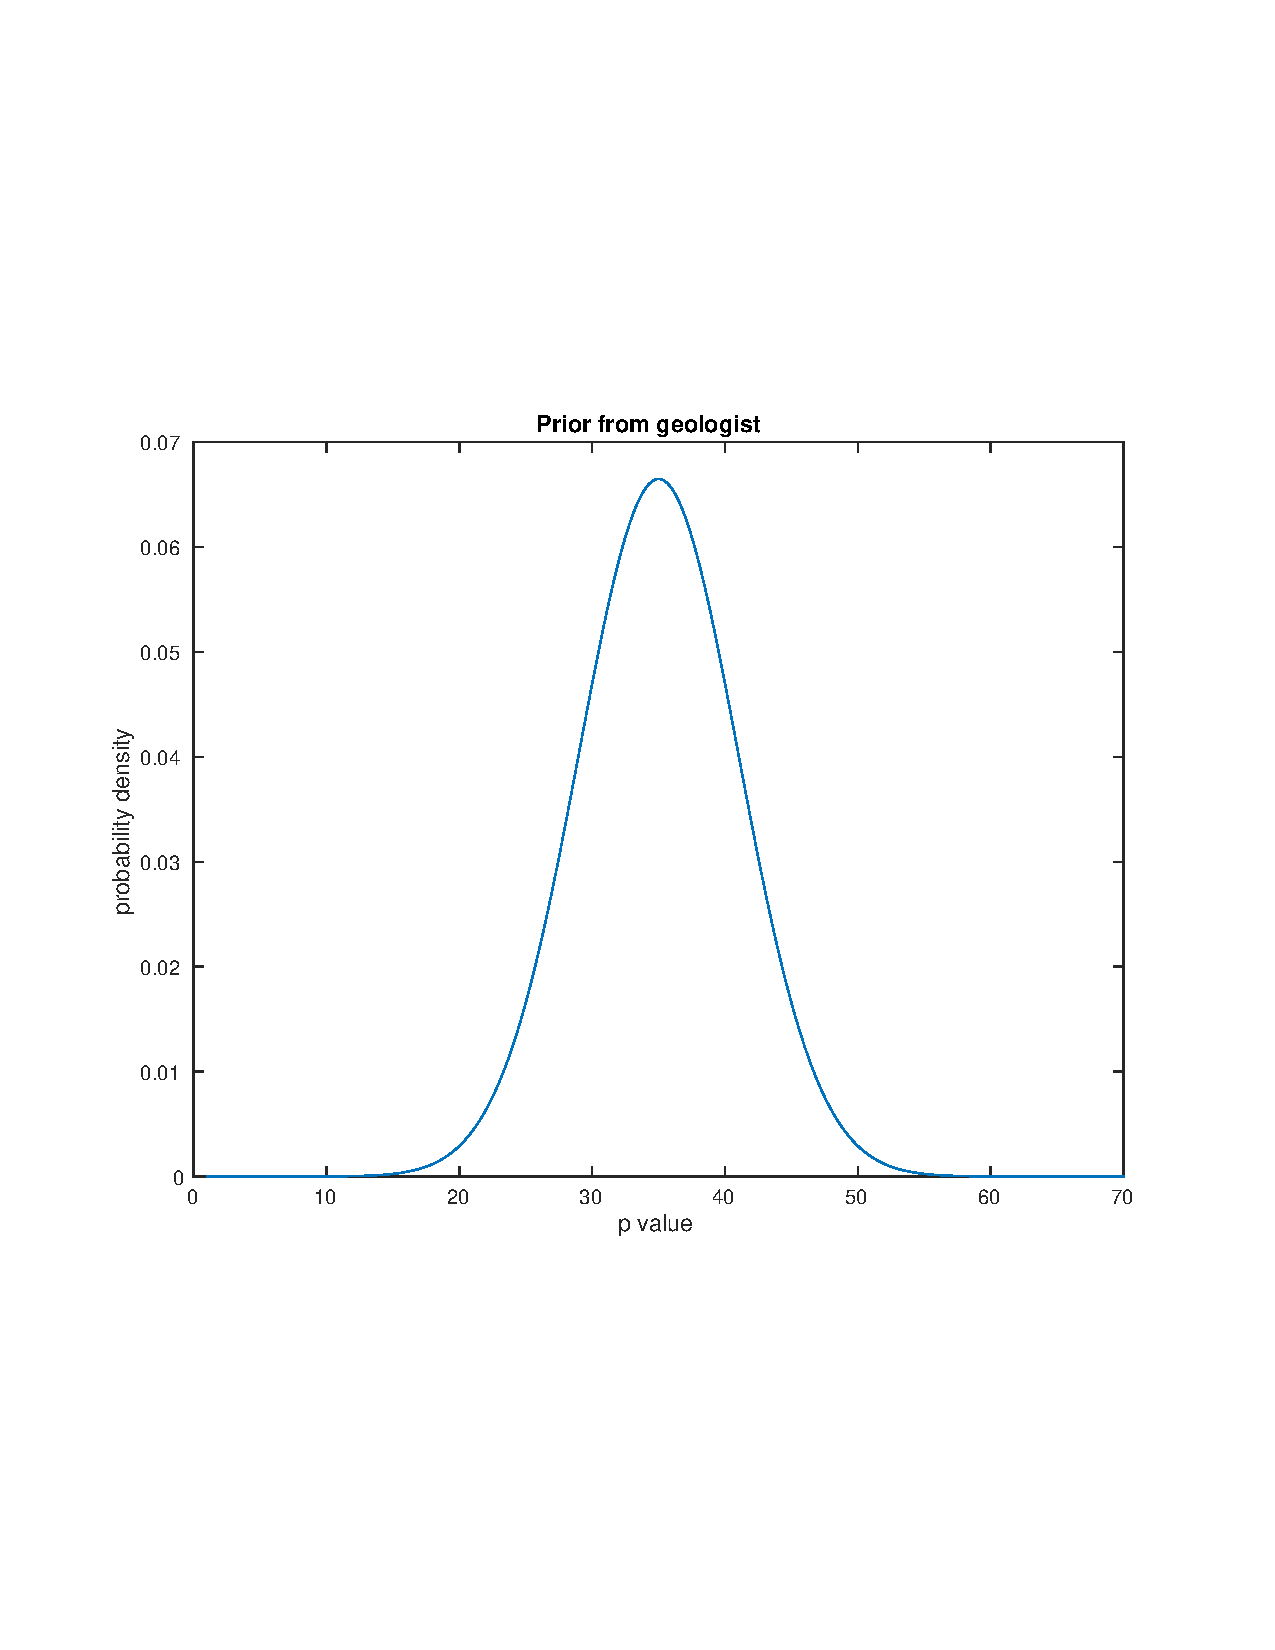
\includegraphics[width=12cm]{Q2/Geo_prior} \caption{Plot of the Gaussian prior for p.}
\end{figure}


\begin{figure}
\centering{}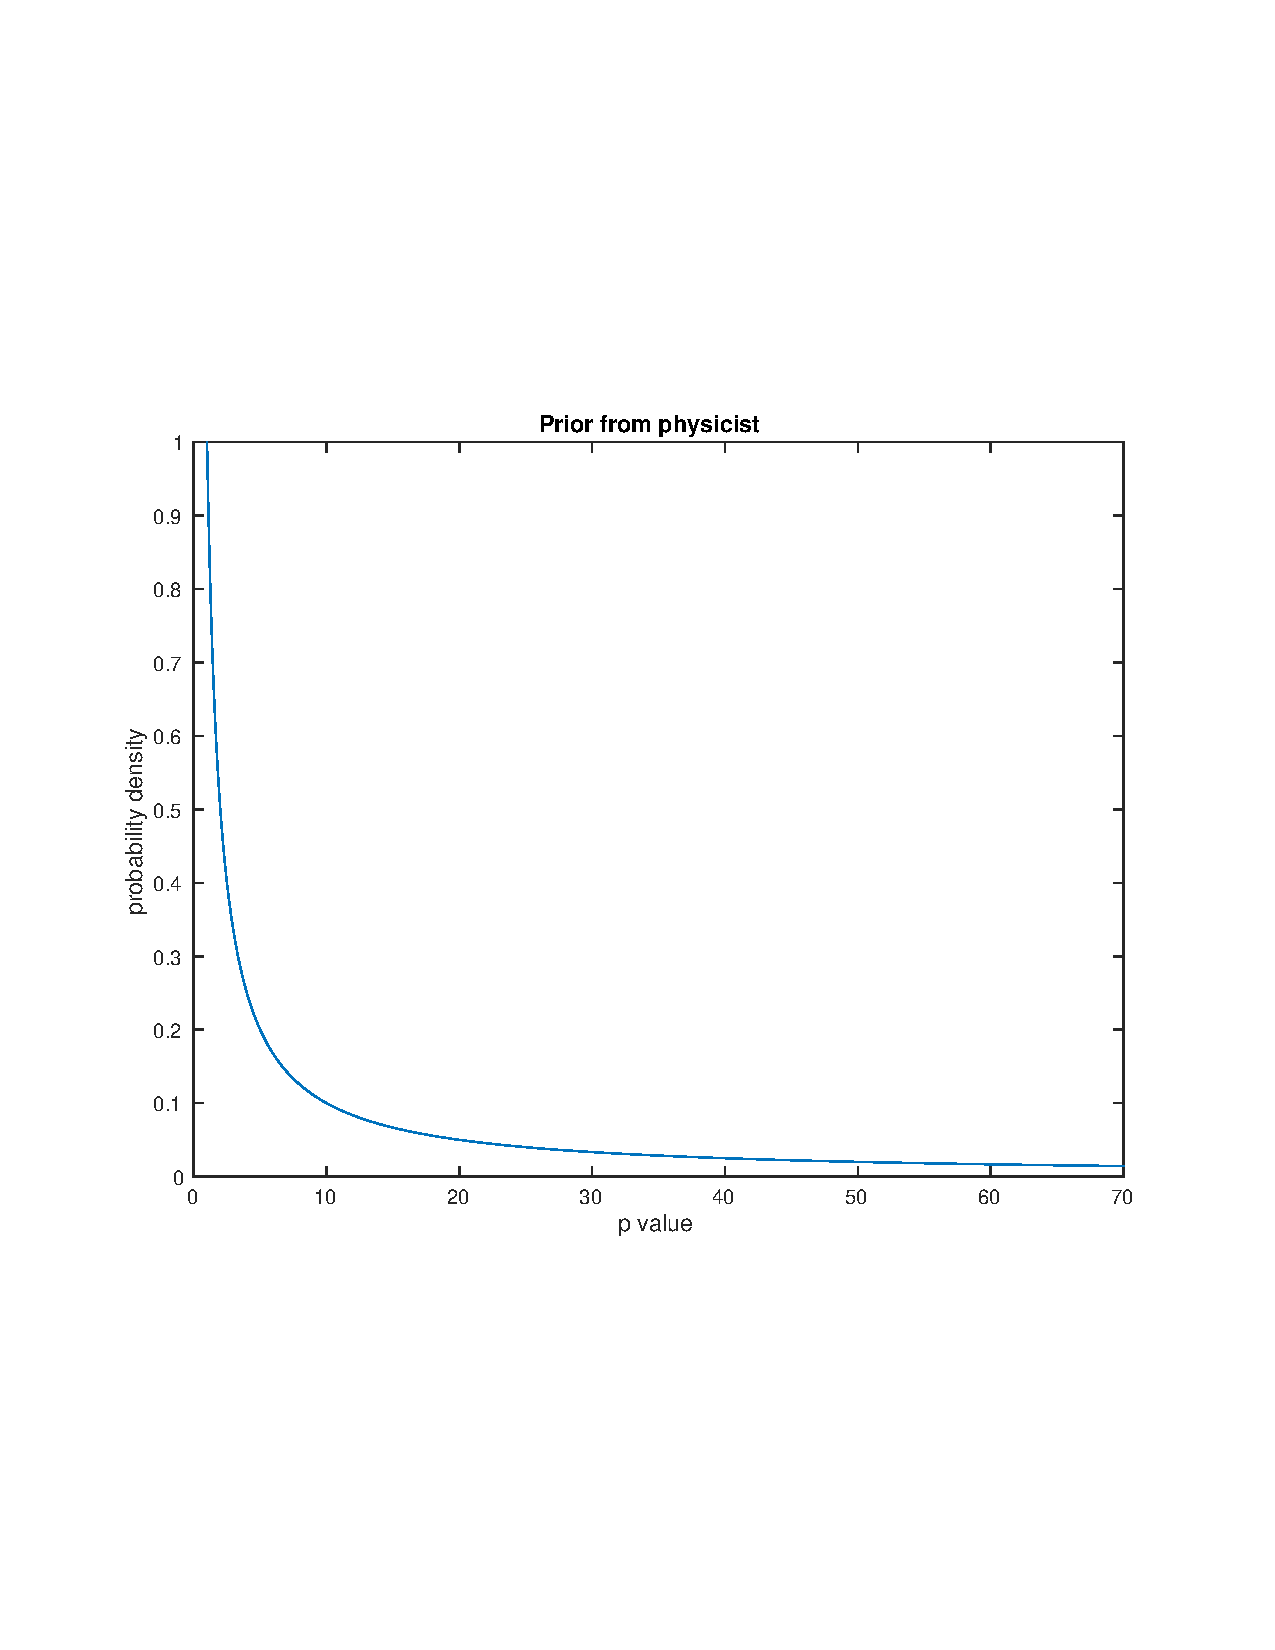
\includegraphics[width=12cm]{Q2/Phy_prior} \caption{Plot of the scale invariant prior for p.}
\end{figure}


\begin{figure}
\centering{}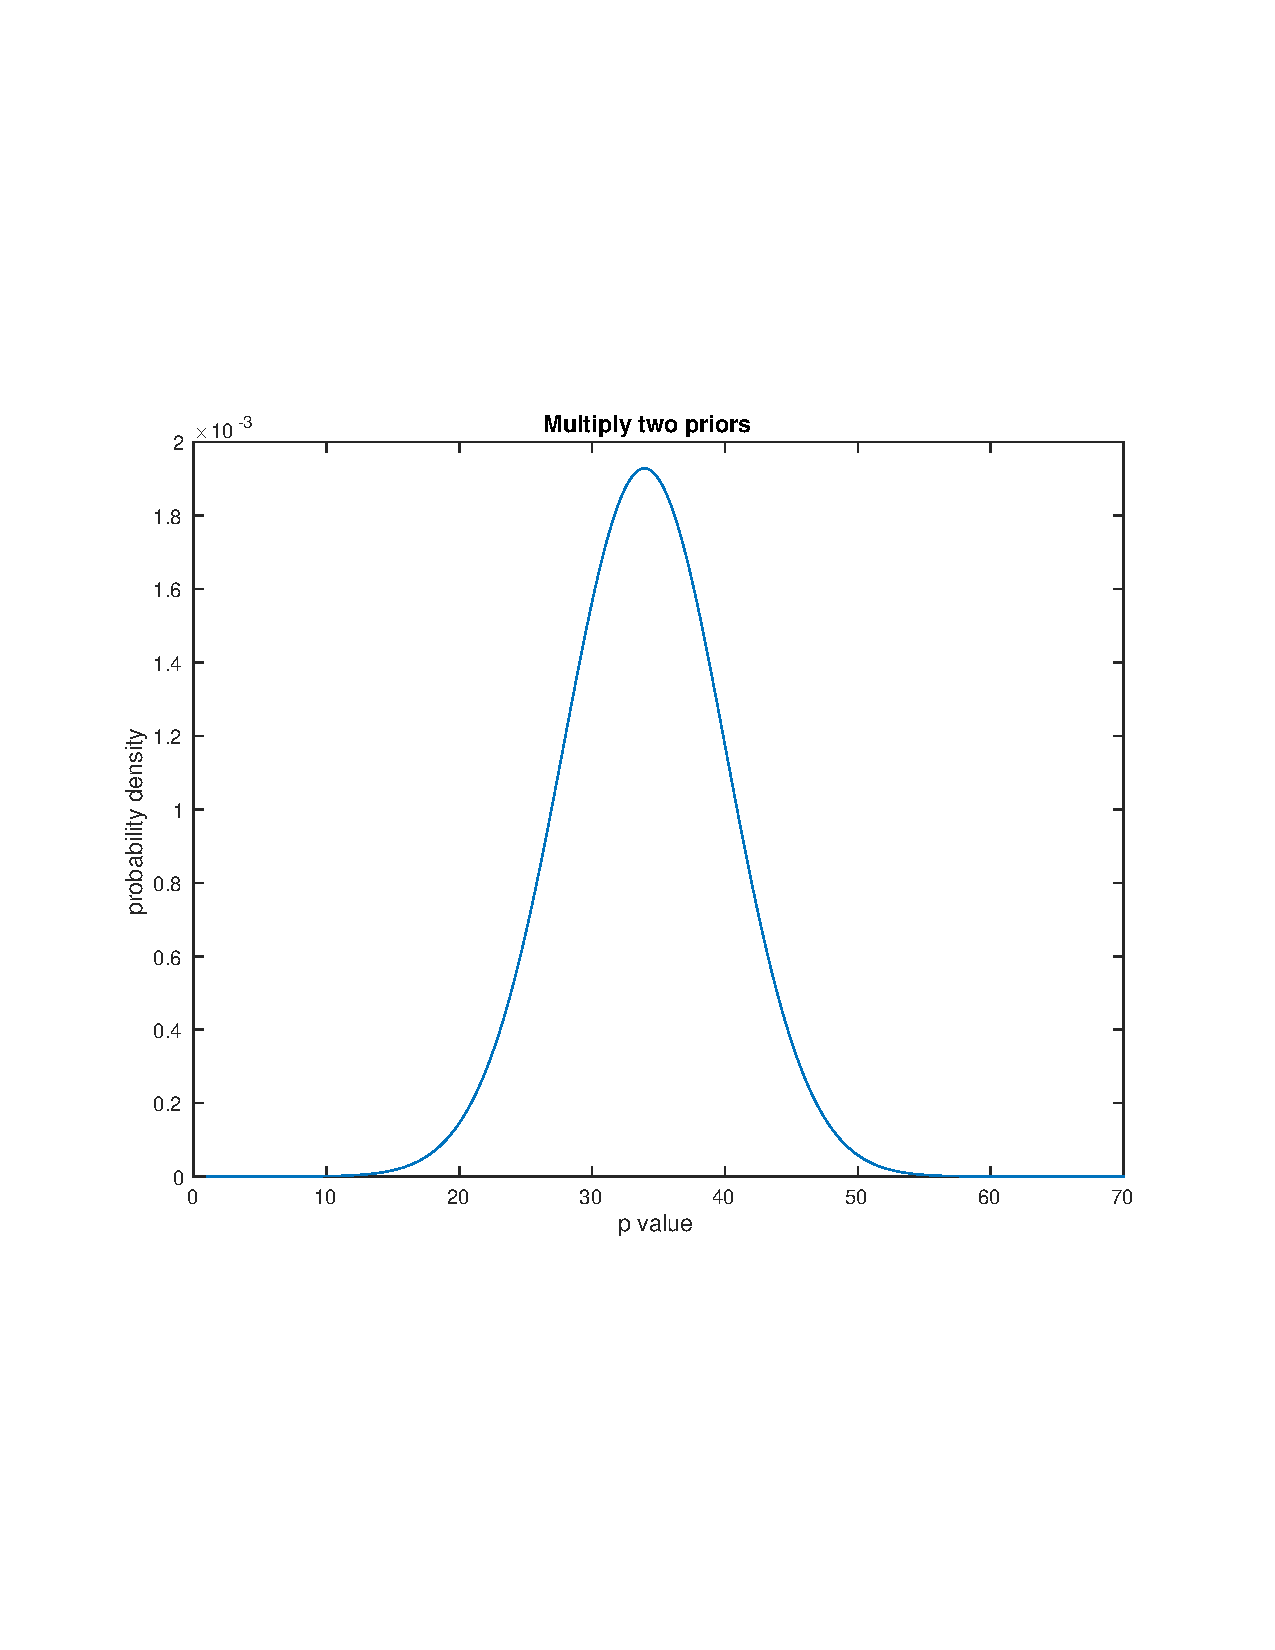
\includegraphics[width=12cm]{Q2/MUl_prior} \caption{Plot of combination of the Gaussian and scale invariant priors for
p. }
\end{figure}



\subsubsection*{(e) - 5 points}

It doesn't matter in what order we do things as long as priors for
analysis are not biased by our data (and they shouldn't be). If we
did the experiment without talking to our friends, we would have no
extra information and would use uniform priors. If we talk to them
first, we use the non-uniform prior we derived in the previous step.


\subsubsection*{(f) - 5 points}

Previous expression: $P_{old}(\boldsymbol{m}|\{d_{k}\})=e^{-F_{old}(\boldsymbol{m})}$
\\
 New expression: $P(\boldsymbol{m}|\{d_{k}\})=\frac{1}{p}e^{-F_{old}(\boldsymbol{m})}e^{-\frac{1}{2}(\frac{p-\mu}{\sigma})^{2}}$
\\


Previous misfit function: $F_{old}(m)$ \\
 To find the new misfit function we will need to manipulate our expression
to get everything into a single exponential. Let's start with the
$\frac{1}{p}$ part:

\begin{eqnarray*}
\frac{1}{p}=e^{(\ln(\frac{1}{p})}=e^{-\ln(p)}\\
P(\boldsymbol{m}|\{d_{k}\})=e^{-\ln(p)}e^{-F_{old}(\boldsymbol{m})}e^{-\frac{1}{2}(\frac{p-\mu}{\sigma})^{2}}\\
\end{eqnarray*}


New misfit function: $F(\boldsymbol{m})=F_{old}(\boldsymbol{m})+\ln(p)+\frac{1}{2}(\frac{p-35}{6})^{2}$
\\


We only need to make a couple simple changes to our code from HW2.
Instead of just using the L2 norm as our error function, we now need
to add our extra two terms to our misfit function:

We will add a term to the last entries of $\gamma$ and the Hessian
to account for the new priors on $p$.

Add the first derivative of our new part of the misfit to $\gamma$:

\begin{eqnarray*}
\gamma=\gamma_{old}-\frac{1}{p}-\frac{p-\mu}{\sigma^{2}}
\end{eqnarray*}


And the second derivative to the last entry of the Hessian:

\begin{eqnarray*}
\frac{\partial^{2}F}{\partial p^{2}}=\frac{\partial^{2}F_{old}}{\partial p^{2}}+\frac{-1}{p^{2}}+\frac{1}{\sigma^{2}}
\end{eqnarray*}


Here is the full code: 


\subsection*{\tiny
\lstinputlisting{./Q2/HW2.m}
\normalsize\tiny
\lstinputlisting{./Q2/compute_gradient_approx_hess.m}
\normalsize\tiny
\lstinputlisting{./Q2/nonlinear_solver.m}
\normalsize\tiny
\lstinputlisting{./Q2/compute_misfit.m}
\normalsize}

Our best fit solution is now: 
\begin{eqnarray*}
m & = & \left(\begin{array}{c}
313.9738\\
30.9907\\
-17.7781\\
21.7237\\
4.9581
\end{array}\right)
\end{eqnarray*}


Our old best fit solution:

\begin{eqnarray*}
m & = & \left(\begin{array}{c}
315.147372215551\\
30.3124982007349\\
-17.1481612373344\\
15.9867180697526\\
5.26992730665649
\end{array}\right)
\end{eqnarray*}


We can see that the addition of these priors did change our solution
for some parameters a small amount (mostly a change in the best fit
for z is observed). As we would expect, the solution for v has been
pushed closer to 4.8 (given our Gaussian prior around this value)
and the other parameters have adjusted accordingly.
\end{document}
